% !TeX program = xelatex
\documentclass[runningheads]{llncs}
\usepackage[paperheight=295mm,paperwidth=210mm]{geometry}
\usepackage{graphicx}
\usepackage{wrapfig}
\usepackage{import}
\usepackage{kotex}
\usepackage[dvipsnames]{xcolor}
\usepackage{fancyvrb} %
\usepackage{listings}
\usepackage{tabularx}
\usepackage{underscore}
\usepackage{multicol}
\usepackage{enumitem}
\usepackage{subcaption}
\usepackage[numbers,square,super]{natbib}
\usepackage{mathptmx} % Times New Roman
\usepackage{amsmath}
\usepackage{amssymb}
\usepackage{framed}
\usepackage{etoolbox}
\usepackage{cancel}
\usepackage{physics}
\usepackage{tikz}
\usepackage{parskip}
\usepackage{enumerate}
\usepackage{minted}
\usepackage{inconsolata}
\usepackage{makecell}
\usepackage{slashed}
\usepackage{nicematrix}
\usetikzlibrary{calc, angles, quotes, graphs, positioning, arrows}

\setcounter{tocdepth}{2}

\colorlet{shadecolor}{gray!30}

\newcommand\enclosebox[2]{%
  \BeforeBeginEnvironment{#1}{\begin{#2}}%
  \AfterEndEnvironment{#1}{\end{#2}}%
}

\enclosebox{theorem}{oframed}
\enclosebox{definition}{leftbar}

\newcommand{\divides}{\bigm|}
\newcommand{\ndivides}{%
  \mathrel{\mkern.5mu % small adjustment
    % superimpose \nmid to \big|
    \ooalign{\hidewidth$\big|$\hidewidth\cr$\nmid$\cr}%
  }%
}
\newcommand{\ord}{\operatorname{\mathrm{ord}}}
\newcommand{\ind}{\operatorname{\mathrm{ind}}}
\newcommand{\legendre}[2]{\left(\frac{#1}{#2}\right)}
\setmainfont{Times New Roman}
\setmainhangulfont{Nanum Myeongjo}
\setmonofont{SF Mono}
\setlength{\parindent}{1em}
\setlength{\parskip}{0pt}
\linespread{1.2}
%\renewcommand{\arraystretch}{1.5}
\setlength{\tabcolsep}{0.5em}%
\newenvironment{Figure}
  {\par\medskip\noindent\minipage{\linewidth}}
  {\endminipage\par\medskip}
\newcommand{\translation}[1]{\textsuperscript{#1}}

\makeatletter
\renewcommand\NAT@citesuper[3]{\ifNAT@swa
\if*#2*\else#2\NAT@spacechar\fi
\unskip\kern\p@\textsuperscript{\NAT@@open#1\if*#3*\else,\NAT@spacechar#3\fi\NAT@@close}%
   \else #1\fi\endgroup}
\makeatother

\let\oldtabular\tabular% Store a copy of \tabular
\let\endoldtabular\endtabular% Store a copy of \endtabular
\renewenvironment{tabular}[2][\arraystretch]
  {\edef\arraystretch{#1}% Update \arraystretch
   \oldtabular{#2}}% \begin{tabular}[<stretch>]{<col spec>}
  {\endoldtabular}% \end{tabular}

\begin{document}

\title{Linear Algebra (0031)\newline\space Project 1}
\author{Yulwon Rhee (202211342)}
\institute{Department of Computer Science and Engineering, Konkuk University}

\maketitle

\subsubsection{1.}
Write a computer program that performs the following:

(a) Take a greyscale image and form a matrix $A$.

(b) For given $n = 2^t, t = 0, 1, \cdots$, construct an $n$-point Haar matrix $H$.

(c) Perform DHWT $B = H^TAH$.

(d) For given $k = 2^s, s = 0, 1, \cdots$, construct an $n \times n$ matrix $\hat{B}$.

(e) Perform the IDHWT $\hat{A} = H\hat{B} H^T$.

(f) Save the reconstructed image $\hat{A}$ into a file.

\captionof{listing}{\texttt{problem1()} from \texttt{prj1.c}}
\begin{minted}[linenos, fontsize=\small, breaklines]{c}
void problem1() {
    BITMAPHEADER outputHeader;
    int imgSize, imgWidth, imgHeight;

    double** A = getImageMatrixFromFileName(&outputHeader, &imgWidth, &imgHeight, &imgSize, "problem1/image_lena_24bit.bmp");

    doDHWT(A, imgHeight, imgWidth, imgSize, outputHeader, "problem1/image_lena_24bit");

    releaseMemory(A, imgHeight);
}
\end{minted}

\captionof{listing}{\texttt{doDHWT()} from \texttt{prj1.c}}
\begin{minted}[linenos, fontsize=\small, breaklines]{c}
void doDHWT(double** originalImageMatrix, int imgHeight, int imgWidth, int imgSize, BITMAPHEADER outputHeader, char** filePathToSave) {
    //Haar matrix H 구성 (orthonormal column을 갖도록 구성)
    int n = imgHeight; //이미지가 정사각형(Height==Width)이라고 가정; n = 2^t,t=0,1,2,...

    // 1. (b)
    double** H = constructHaarMatrixRecursive(n);
    double** normalisedH = normaliseMatrix(H, n, n);

    // 1. (c)
    double** transposedNormalisedH = transposeMatrix(normalisedH, n, n);
    double** HTA = multiplyTwoMatrices(transposedNormalisedH, n, n, originalImageMatrix, n, n);
    double** B = multiplyTwoMatrices(HTA, n, n, normalisedH, n, n);

    // 1. (d)
    double** Bhat = allocateMemory(imgHeight, imgWidth);

    for (int s = 0; s <= 9; s++) { // 2^9 = 512
        int k = pow(2, s);

        // Construct Matrix B Hat
        for (int i = 0; i < imgHeight; i++) {
            for (int j = 0; j < imgWidth; j++) {
                if (i < k && j < k) Bhat[i][j] = B[i][j];
                else Bhat[i][j] = 0;
            }
        }

        // 1. (e)
        double** HBhat = multiplyTwoMatrices(normalisedH, n, n, Bhat, n, n);
        double** Ahat = multiplyTwoMatrices(HBhat, n, n, transposedNormalisedH, n, n);

        // 1. (f)
        // Write Reconstructed Image
        // Ahat을 이용해서 위의 image와 같은 형식이 되도록 구성 (즉, Ahat = [a b;c d]면 [a a a b b b c c c d d d]를 만들어야 함)
        BYTE* Are = (BYTE*)malloc(BYTES_PER_PIXEL * sizeof(BYTE) * imgSize);

        for (int i = 0; i < imgHeight; i++)
            for (int j = 0; j < imgWidth; j++)
                for (int k = 0; k < BYTES_PER_PIXEL; k++)
                    Are[(i * imgWidth + j) * BYTES_PER_PIXEL + k] = (BYTE)Ahat[i][j];

        char fileName[50] = "";
        strcat(fileName, filePathToSave);
        strcat(fileName, "_");
        char kStr[5];
        sprintf(kStr, "%d", k);
        strcat(fileName, kStr);
        strcat(fileName, ".bmp");

        writeBitmapFile(BYTES_PER_PIXEL, outputHeader, Are, imgSize, fileName);
        printf("%s saved.\n", fileName);

        releaseMemory(HBhat, n);
        releaseMemory(Ahat, n);
        free(Are);
    }

    releaseMemory(H, n);
    releaseMemory(normalisedH, n);
    releaseMemory(transposedNormalisedH, n);
    releaseMemory(HTA, n);
    releaseMemory(B, n);
    releaseMemory(Bhat, n);
}
\end{minted}

\captionof{listing}{\texttt{getImageMatrixFromFileName()} from \texttt{bitmapManager.h}}
\begin{minted}[linenos, fontsize=\small, breaklines]{c}
double** getImageMatrixFromFileName(BITMAPHEADER* outputHeader, int* imgWidth, int* imgHeight, int* imgSize, char* filePath) {
    BITMAPHEADER originalHeader;
    BYTE* image = loadBitmapFile(BYTES_PER_PIXEL, &originalHeader, imgWidth, imgHeight, filePath);

    if (image == NULL) return 0;

    *imgSize = *imgWidth * *imgHeight;
    BYTE* output = (BYTE*)malloc(BYTES_PER_PIXEL * sizeof(BYTE) * *imgSize);
    *outputHeader = originalHeader;

    double** A = allocateMemory(*imgHeight, *imgWidth);

    for (int i = 0; i < *imgHeight; i++)
        for (int j = 0; j < *imgWidth; j++)
            A[i][j] = (double)image[(i * *imgWidth + j) * BYTES_PER_PIXEL];

    free(image);
    free(output);

    return A;
}   
\end{minted}
\newpage
\begin{figure}[H]
    \centering
    \caption{Result Images After DHWT}
    \begin{subfigure}[b]{0.3\textwidth}
        \centering
        \includegraphics[width=\textwidth]{problem1/image_lena_24bit_1.bmp}
        \caption{$k = 2^0$}
    \end{subfigure}
    \hfill
    \begin{subfigure}[b]{0.3\textwidth}
        \centering
        \includegraphics[width=\textwidth]{problem1/image_lena_24bit_2.bmp}
        \caption{$k = 2^1$}
    \end{subfigure}
    \hfill
    \begin{subfigure}[b]{0.3\textwidth}
        \centering
        \includegraphics[width=\textwidth]{problem1/image_lena_24bit_4.bmp}
        \caption{$k = 2^2$}
    \end{subfigure}
    \begin{subfigure}[b]{0.3\textwidth}
        \centering
        \includegraphics[width=\textwidth]{problem1/image_lena_24bit_8.bmp}
        \caption{$k = 2^3$}
    \end{subfigure}
    \hfill
    \begin{subfigure}[b]{0.3\textwidth}
        \centering
        \includegraphics[width=\textwidth]{problem1/image_lena_24bit_16.bmp}
        \caption{$k = 2^4$}
    \end{subfigure}
    \hfill
    \begin{subfigure}[b]{0.3\textwidth}
        \centering
        \includegraphics[width=\textwidth]{problem1/image_lena_24bit_32.bmp}
        \caption{$k = 2^5$}
    \end{subfigure}
    \begin{subfigure}[b]{0.3\textwidth}
        \centering
        \includegraphics[width=\textwidth]{problem1/image_lena_24bit_64.bmp}
        \caption{$k = 2^6$}
    \end{subfigure}
    \hfill
    \begin{subfigure}[b]{0.3\textwidth}
        \centering
        \includegraphics[width=\textwidth]{problem1/image_lena_24bit_128.bmp}
        \caption{$k = 2^7$}
    \end{subfigure}
    \hfill
    \begin{subfigure}[b]{0.3\textwidth}
        \centering
        \includegraphics[width=\textwidth]{problem1/image_lena_24bit_256.bmp}
        \caption{$k = 2^8$}
    \end{subfigure}
    \begin{subfigure}[b]{0.3\textwidth}
        \centering
        \includegraphics[width=\textwidth]{problem1/image_lena_24bit_512.bmp}
        \caption{$k = 2^9$}
    \end{subfigure}
    \hfill
    \begin{subfigure}[b]{0.3\textwidth}
        \centering
        \includegraphics[width=\textwidth]{problem1/image_lena_24bit.bmp}
        \caption{Original Image}
    \end{subfigure}
\end{figure}
\newpage
\subsubsection{2.} Get any 2 grayscale images of any format from anywhere (Internet, your personal photos, etc.). It is recommended that you get one image with low frequency components, and one image filled with high frequency components. Use your computer program to do the following:

(a) As $k$ increases, observe the quality of reconstructed image.

(b) Describe any difference between low-freq. image and high-freq. image.

(c) Discuss any findings or thoughts.

\captionof{listing}{\texttt{problem2()} from \texttt{prj1.c}}
\begin{minted}[linenos, fontsize=\small, breaklines]{c}
void problem2() {
    BITMAPHEADER lowFreqOutputHeader, highFreqOutputHeader;
    int lowFreqWidth, lowFreqHeight, lowFreqSize, highFreqWidth, highFreqHeight, highFreqSize;

    double** lowFreqImgMatrix = getImageMatrixFromFileName(&lowFreqOutputHeader,
        &lowFreqWidth,
        &lowFreqHeight,
        &lowFreqSize,
        "problem2/low_freq.bmp");

    doDHWT(lowFreqImgMatrix, lowFreqHeight, lowFreqWidth, lowFreqSize, lowFreqOutputHeader, "problem2/low_freq");


    double** highFreqImgMatrix = getImageMatrixFromFileName(&highFreqOutputHeader,
        &highFreqWidth,
        &highFreqHeight,
        &highFreqSize,
        "problem2/high_freq.bmp");

    doDHWT(highFreqImgMatrix, highFreqHeight, highFreqWidth, highFreqSize, highFreqOutputHeader, "problem2/high_freq");

    releaseMemory(lowFreqImgMatrix, lowFreqHeight);
    releaseMemory(highFreqImgMatrix, highFreqHeight);
}
\end{minted}
\pagebreak
\begin{figure}[H]
    \centering
    \caption{Result of Low Frequency Image After DHWT}
    \begin{subfigure}[b]{0.3\textwidth}
        \centering
        \includegraphics[width=\textwidth]{problem2/low_freq_1.bmp}
        \caption{$k = 2^0$}
    \end{subfigure}
    \hfill
    \begin{subfigure}[b]{0.3\textwidth}
        \centering
        \includegraphics[width=\textwidth]{problem2/low_freq_2.bmp}
        \caption{$k = 2^1$}
    \end{subfigure}
    \hfill
    \begin{subfigure}[b]{0.3\textwidth}
        \centering
        \includegraphics[width=\textwidth]{problem2/low_freq_4.bmp}
        \caption{$k = 2^2$}
    \end{subfigure}
    \begin{subfigure}[b]{0.3\textwidth}
        \centering
        \includegraphics[width=\textwidth]{problem2/low_freq_8.bmp}
        \caption{$k = 2^3$}
    \end{subfigure}
    \hfill
    \begin{subfigure}[b]{0.3\textwidth}
        \centering
        \includegraphics[width=\textwidth]{problem2/low_freq_16.bmp}
        \caption{$k = 2^4$}
    \end{subfigure}
    \hfill
    \begin{subfigure}[b]{0.3\textwidth}
        \centering
        \includegraphics[width=\textwidth]{problem2/low_freq_32.bmp}
        \caption{$k = 2^5$}
    \end{subfigure}
    \begin{subfigure}[b]{0.3\textwidth}
        \centering
        \includegraphics[width=\textwidth]{problem2/low_freq_64.bmp}
        \caption{$k = 2^6$}
    \end{subfigure}
    \hfill
    \begin{subfigure}[b]{0.3\textwidth}
        \centering
        \includegraphics[width=\textwidth]{problem2/low_freq_128.bmp}
        \caption{$k = 2^7$}
    \end{subfigure}
    \hfill
    \begin{subfigure}[b]{0.3\textwidth}
        \centering
        \includegraphics[width=\textwidth]{problem2/low_freq_256.bmp}
        \caption{$k = 2^8$}
    \end{subfigure}
    \begin{subfigure}[b]{0.3\textwidth}
        \centering
        \includegraphics[width=\textwidth]{problem2/low_freq_512.bmp}
        \caption{$k = 2^9$}
    \end{subfigure}
    \hfill
    \begin{subfigure}[b]{0.3\textwidth}
        \centering
        \includegraphics[width=\textwidth]{problem2/low_freq.bmp}
        \caption{Original Image}
    \end{subfigure}
\end{figure}
\pagebreak
\begin{figure}[H]
    \centering
    \caption{Result of High Frequency Image After DHWT}
    \begin{subfigure}[b]{0.3\textwidth}
        \centering
        \includegraphics[width=\textwidth]{problem2/high_freq_1.bmp}
        \caption{$k = 2^0$}
    \end{subfigure}
    \hfill
    \begin{subfigure}[b]{0.3\textwidth}
        \centering
        \includegraphics[width=\textwidth]{problem2/high_freq_2.bmp}
        \caption{$k = 2^1$}
    \end{subfigure}
    \hfill
    \begin{subfigure}[b]{0.3\textwidth}
        \centering
        \includegraphics[width=\textwidth]{problem2/high_freq_4.bmp}
        \caption{$k = 2^2$}
    \end{subfigure}
    \begin{subfigure}[b]{0.3\textwidth}
        \centering
        \includegraphics[width=\textwidth]{problem2/high_freq_8.bmp}
        \caption{$k = 2^3$}
    \end{subfigure}
    \hfill
    \begin{subfigure}[b]{0.3\textwidth}
        \centering
        \includegraphics[width=\textwidth]{problem2/high_freq_16.bmp}
        \caption{$k = 2^4$}
    \end{subfigure}
    \hfill
    \begin{subfigure}[b]{0.3\textwidth}
        \centering
        \includegraphics[width=\textwidth]{problem2/high_freq_32.bmp}
        \caption{$k = 2^5$}
    \end{subfigure}
    \begin{subfigure}[b]{0.3\textwidth}
        \centering
        \includegraphics[width=\textwidth]{problem2/high_freq_64.bmp}
        \caption{$k = 2^6$}
    \end{subfigure}
    \hfill
    \begin{subfigure}[b]{0.3\textwidth}
        \centering
        \includegraphics[width=\textwidth]{problem2/high_freq_128.bmp}
        \caption{$k = 2^7$}
    \end{subfigure}
    \hfill
    \begin{subfigure}[b]{0.3\textwidth}
        \centering
        \includegraphics[width=\textwidth]{problem2/high_freq_256.bmp}
        \caption{$k = 2^8$}
    \end{subfigure}
    \begin{subfigure}[b]{0.3\textwidth}
        \centering
        \includegraphics[width=\textwidth]{problem2/high_freq_512.bmp}
        \caption{$k = 2^9$}
    \end{subfigure}
    \hfill
    \begin{subfigure}[b]{0.3\textwidth}
        \centering
        \includegraphics[width=\textwidth]{problem2/high_freq.bmp}
        \caption{Original Image}
    \end{subfigure}
\end{figure}
High frequency image의 경우, $k$의 값이 낮아질 수록 품질이 급격하게 하락하여 $k = 2^7$인 경우 글자를 읽을 수 없게 되고,
$k = 2^6$부터는 사물을 정확히 판별하기 어려워진다.
반면 Low frequency image의 경우, $k$의 값이 낮아지더라도 크게 품질이 하락하지 않으며, 위 이미지의 $k=2^6$인 경우에도 원본과 큰 차이 없이 형체를 인식할 수 있다.

\subsubsection{3.} (a), (b), (c), (d)
\captionof{listing}{\texttt{problem3()} from \texttt{prj1.c}}
\begin{minted}[linenos, fontsize=\small, breaklines]{c}
void problem3() {
    BITMAPHEADER outputHeader;
    int imgSize, imgWidth, imgHeight;

    double** A = getImageMatrixFromFileName(&outputHeader, &imgWidth, &imgHeight, &imgSize, "problem3/image_lena_24bit.bmp");

    int n = imgHeight;

    // Split H^T into H_l and H_h
    double** H = constructHaarMatrixRecursive(n);
    double** normalisedH = normaliseMatrix(H, n, n);
    double** transposedNormalisedH = transposeMatrix(normalisedH, n, n);

    double** Hl = allocateMemory(n / 2, n);
    double** Hh = allocateMemory(n / 2, n);

    for (int i = 0; i < n; i++) {
        for (int j = 0; j < n; j++) {
            if (i < n / 2) Hl[i][j] = transposedNormalisedH[i][j];
            else Hh[i - n / 2][j] = transposedNormalisedH[i][j];
        }
    }
    double** HlT = transposeMatrix(Hl, n / 2, n);
    double** HhT = transposeMatrix(Hh, n / 2, n);

    // 3. (a) LHS
    double** HTA = multiplyTwoMatrices(transposedNormalisedH, n, n, A, n, n);
    double** B = multiplyTwoMatrices(HTA, n, n, normalisedH, n, n);

    // 3. (a) RHS
    double** HlA = multiplyTwoMatrices(Hl, n / 2, n, A, n, n);
    double** HhA = multiplyTwoMatrices(Hh, n / 2, n, A, n, n);

    double** HlAHlT = multiplyTwoMatrices(HlA, n / 2, n, HlT, n, n / 2);
    double** HlAHhT = multiplyTwoMatrices(HlA, n / 2, n, HhT, n, n / 2);
    double** HhAHlT = multiplyTwoMatrices(HhA, n / 2, n, HlT, n, n / 2);
    double** HhAHhT = multiplyTwoMatrices(HhA, n / 2, n, HhT, n, n / 2);

    // 3. (a) Check LHS == RHS
    bool isASame = true;
    for (int i = 0; i < n; i++) {
        for (int j = 0; j < n; j++) {
            double cmp = 0;
            if (i < n / 2 && j < n / 2) cmp = HlAHlT[i][j];
            else if (i < n / 2 && j >= n / 2) cmp = HlAHhT[i][j - n / 2];
            else if (i >= n / 2 && j < n / 2) cmp = HhAHlT[i - n / 2][j];
            else cmp = HhAHhT[i - n / 2][j - n / 2];

            if (!doubleEquals(cmp, B[i][j])) isASame = false;
        }
    }

    printf("3. (a): %s\n", isASame ? "true" : "false");


    // 3. (b) LHS
    double** HB = multiplyTwoMatrices(normalisedH, n, n, B, n, n);
    double** HBHT = multiplyTwoMatrices(HB, n, n, transposedNormalisedH, n, n);

    // 3. (b) RHS
    double** HlTHlAHlT = multiplyTwoMatrices(HlT, n, n / 2, HlAHlT, n / 2, n / 2);
    double** HlTHlAHlTHl = multiplyTwoMatrices(HlTHlAHlT, n, n / 2, Hl, n / 2, n);

    double** HlTHlAHhT = multiplyTwoMatrices(HlT, n, n / 2, HlAHhT, n / 2, n / 2);
    double** HlTHlAHhTHh = multiplyTwoMatrices(HlTHlAHhT, n, n / 2, Hh, n / 2, n);

    double** HhTHhAHlT = multiplyTwoMatrices(HhT, n, n / 2, HhAHlT, n / 2, n / 2);
    double** HhTHhAHlTHl = multiplyTwoMatrices(HhTHhAHlT, n, n / 2, Hl, n / 2, n);

    double** HhTHhAHhT = multiplyTwoMatrices(HhT, n, n / 2, HhAHhT, n / 2, n / 2);
    double** HhTHhAHhTHh = multiplyTwoMatrices(HhTHhAHhT, n, n / 2, Hh, n / 2, n);

    double** LURU = addTwoMatrices(HlTHlAHlTHl, n, n, HlTHlAHhTHh, n, n);
    double** LURULL = addTwoMatrices(LURU, n, n, HhTHhAHlTHl, n, n);
    double** RHS = addTwoMatrices(LURULL, n, n, HhTHhAHhTHh, n, n);

    // 3. (b) Check LHS == RHS
    bool isBSame = true;
    for (int i = 0; i < n; i++) {
        for (int j = 0; j < n; j++) {
            if (!doubleEquals(HBHT[i][j], RHS[i][j])) isBSame = false;
        }
    }

    printf("3. (b): %s\n", isBSame ? "true" : "false");

    // 3. (c)
    BYTE* term1 = (BYTE*)malloc(BYTES_PER_PIXEL * sizeof(BYTE) * imgSize);
    
    for (int i = 0; i < imgHeight; i++)
        for (int j = 0; j < imgWidth; j++)
            for (int k = 0; k < BYTES_PER_PIXEL; k++)
                term1[(i * imgWidth + j) * BYTES_PER_PIXEL + k] = (BYTE)HlTHlAHlTHl[i][j];

    writeBitmapFile(BYTES_PER_PIXEL, outputHeader, term1, imgSize, "problem3/term1.bmp");


    BYTE* term2 = (BYTE*)malloc(BYTES_PER_PIXEL * sizeof(BYTE) * imgSize);

    for (int i = 0; i < imgHeight; i++)
        for (int j = 0; j < imgWidth; j++)
            for (int k = 0; k < BYTES_PER_PIXEL; k++)
                term2[(i * imgWidth + j) * BYTES_PER_PIXEL + k] = (BYTE)HlTHlAHhTHh[i][j];

    writeBitmapFile(BYTES_PER_PIXEL, outputHeader, term2, imgSize, "problem3/term2.bmp");


    BYTE* term3 = (BYTE*)malloc(BYTES_PER_PIXEL * sizeof(BYTE) * imgSize);

    for (int i = 0; i < imgHeight; i++)
        for (int j = 0; j < imgWidth; j++)
            for (int k = 0; k < BYTES_PER_PIXEL; k++)
                term3[(i * imgWidth + j) * BYTES_PER_PIXEL + k] = (BYTE)HhTHhAHlTHl[i][j];

    writeBitmapFile(BYTES_PER_PIXEL, outputHeader, term3, imgSize, "problem3/term3.bmp");


    BYTE* term4 = (BYTE*)malloc(BYTES_PER_PIXEL * sizeof(BYTE) * imgSize);

    for (int i = 0; i < imgHeight; i++)
        for (int j = 0; j < imgWidth; j++)
            for (int k = 0; k < BYTES_PER_PIXEL; k++)
                term4[(i * imgWidth + j) * BYTES_PER_PIXEL + k] = (BYTE)HhTHhAHhTHh[i][j];

    writeBitmapFile(BYTES_PER_PIXEL, outputHeader, term4, imgSize, "problem3/term4.bmp");

    
    // 3. (d)

    double** Hll = allocateMemory(n / 4, n);
    double** Hlh = allocateMemory(n / 4, n);

    for (int i = 0; i < n / 2; i++) {
        for (int j = 0; j < n; j++) {
            if (i < n / 4) Hll[i][j] = Hl[i][j];
            else Hlh[i - n / 4][j] = Hl[i][j];
        }
    }

    double** HllT = transposeMatrix(Hll, n / 4, n);
    double** HlhT = transposeMatrix(Hlh, n / 4, n);

    // 3. (d) RHS
    double** HllA = multiplyTwoMatrices(Hll, n / 4, n, A, n, n);
    double** HlhA = multiplyTwoMatrices(Hlh, n / 4, n, A, n, n);

    double** HllAHllT = multiplyTwoMatrices(HllA, n / 4, n, HllT, n, n / 4);
    double** HllAHlhT = multiplyTwoMatrices(HllA, n / 4, n, HlhT, n, n / 4);
    double** HlhAHllT = multiplyTwoMatrices(HlhA, n / 4, n, HllT, n, n / 4);
    double** HlhAHlhT = multiplyTwoMatrices(HlhA, n / 4, n, HlhT, n, n / 4);
    
    double** HllTHllAHllT = multiplyTwoMatrices(HllT, n, n / 4, HllAHllT, n / 4, n / 4);
    double** HllTHllAHllTHll = multiplyTwoMatrices(HllTHllAHllT, n, n / 4, Hll, n / 4, n);

    double** HllTHllAHlhT = multiplyTwoMatrices(HllT, n, n / 4, HllAHlhT, n / 4, n / 4);
    double** HllTHllAHlhTHlh = multiplyTwoMatrices(HllTHllAHlhT, n, n / 4, Hlh, n / 4, n);

    double** HlhTHlhAHllT = multiplyTwoMatrices(HlhT, n, n / 4, HlhAHllT, n / 4, n / 4);
    double** HlhTHlhAHllTHll = multiplyTwoMatrices(HlhTHlhAHllT, n, n / 4, Hll, n / 4, n);

    double** HlhTHlhAHlhT = multiplyTwoMatrices(HlhT, n, n / 4, HlhAHlhT, n / 4, n / 4);
    double** HlhTHlhAHlhTHlh = multiplyTwoMatrices(HlhTHlhAHlhT, n, n / 4, Hlh, n / 4, n);

    double** dLURU = addTwoMatrices(HllTHllAHllTHll, n, n, HllTHllAHlhTHlh, n, n);
    double** dLURULL = addTwoMatrices(dLURU, n, n, HlhTHlhAHllTHll, n, n);
    double** dRHS = addTwoMatrices(dLURULL, n, n, HlhTHlhAHlhTHlh, n, n);

    // 3. (d) Check LHS == RHS
    bool isDSame = true;
    for (int i = 0; i < n; i++) {
        for (int j = 0; j < n; j++) {
            if (!doubleEquals(HlTHlAHlTHl[i][j], dRHS[i][j])) isDSame = false;
        }
    }

    printf("3. (d): %s\n", isDSame ? "true" : "false");

    // 3. (d) Save Image
    BYTE* dTerm1 = (BYTE*)malloc(BYTES_PER_PIXEL * sizeof(BYTE) * imgSize);

    for (int i = 0; i < imgHeight; i++)
        for (int j = 0; j < imgWidth; j++)
            for (int k = 0; k < BYTES_PER_PIXEL; k++)
                dTerm1[(i * imgWidth + j) * BYTES_PER_PIXEL + k] = (BYTE)HllTHllAHllTHll[i][j];

    writeBitmapFile(BYTES_PER_PIXEL, outputHeader, dTerm1, imgSize, "problem3/dTerm1.bmp");


    BYTE* dTerm2 = (BYTE*)malloc(BYTES_PER_PIXEL * sizeof(BYTE) * imgSize);

    for (int i = 0; i < imgHeight; i++)
        for (int j = 0; j < imgWidth; j++)
            for (int k = 0; k < BYTES_PER_PIXEL; k++)
                dTerm2[(i * imgWidth + j) * BYTES_PER_PIXEL + k] = (BYTE)HllTHllAHlhTHlh[i][j];

    writeBitmapFile(BYTES_PER_PIXEL, outputHeader, dTerm2, imgSize, "problem3/dTerm2.bmp");


    BYTE* dTerm3 = (BYTE*)malloc(BYTES_PER_PIXEL * sizeof(BYTE) * imgSize);

    for (int i = 0; i < imgHeight; i++)
        for (int j = 0; j < imgWidth; j++)
            for (int k = 0; k < BYTES_PER_PIXEL; k++)
                dTerm3[(i * imgWidth + j) * BYTES_PER_PIXEL + k] = (BYTE)HlhTHlhAHllTHll[i][j];

    writeBitmapFile(BYTES_PER_PIXEL, outputHeader, dTerm3, imgSize, "problem3/dTerm3.bmp");


    BYTE* dTerm4 = (BYTE*)malloc(BYTES_PER_PIXEL * sizeof(BYTE) * imgSize);

    for (int i = 0; i < imgHeight; i++)
        for (int j = 0; j < imgWidth; j++)
            for (int k = 0; k < BYTES_PER_PIXEL; k++)
                dTerm4[(i * imgWidth + j) * BYTES_PER_PIXEL + k] = (BYTE)HlhTHlhAHlhTHlh[i][j];

    writeBitmapFile(BYTES_PER_PIXEL, outputHeader, dTerm4, imgSize, "problem3/dTerm4.bmp");

    
    // Release Allocated Memory
    free(dTerm4);
    free(dTerm3);
    free(dTerm2);
    free(dTerm1);
    releaseMemory(HllA, n / 4);
    releaseMemory(HllAHllT, n / 4);
    releaseMemory(HllAHlhT, n / 4);
    releaseMemory(HlhAHllT, n / 4);
    releaseMemory(HlhAHlhT, n / 4);
    releaseMemory(HllTHllAHllT, n);
    releaseMemory(HllTHllAHllTHll, n);
    releaseMemory(HllTHllAHlhT, n);
    releaseMemory(HllTHllAHlhTHlh, n);
    releaseMemory(HlhTHlhAHllT, n);
    releaseMemory(HlhTHlhAHllTHll, n);
    releaseMemory(HlhTHlhAHlhT, n);
    releaseMemory(HlhTHlhAHlhTHlh, n);
    releaseMemory(dLURU, n);
    releaseMemory(dLURULL, n);
    releaseMemory(dRHS, n);
    free(term4);
    free(term3);
    free(term2);
    free(term1);
    releaseMemory(RHS, n);
    releaseMemory(LURULL, n);
    releaseMemory(LURU, n);
    releaseMemory(HhTHhAHhTHh, n);
    releaseMemory(HhTHhAHhT, n);
    releaseMemory(HhTHhAHlTHl, n);
    releaseMemory(HhTHhAHlT, n);
    releaseMemory(HlTHlAHhTHh, n);
    releaseMemory(HlTHlAHhT, n);
    releaseMemory(HlTHlAHlTHl, n);
    releaseMemory(HlTHlAHlT, n);
    releaseMemory(HBHT, n);
    releaseMemory(HB, n);
    releaseMemory(HhAHhT, n / 2);
    releaseMemory(HhAHlT, n / 2);
    releaseMemory(HlAHhT, n / 2);
    releaseMemory(HlAHlT, n / 2);
    releaseMemory(HhA, n / 2);
    releaseMemory(HlA, n / 2);
    releaseMemory(B, n);
    releaseMemory(HTA, n);
    releaseMemory(Hh, n / 2);
    releaseMemory(Hl, n / 2);
    releaseMemory(transposedNormalisedH, n);
    releaseMemory(normalisedH, n);
    releaseMemory(H, n);
    
}
\end{minted}
\begin{figure}[H]
    \centering
    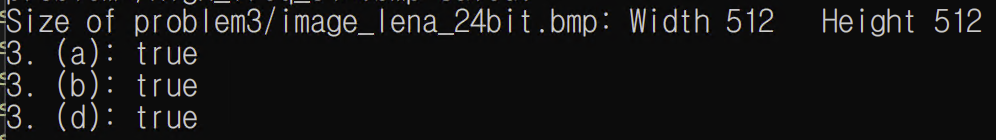
\includegraphics{execution.png}
    \caption{Program Execution Result}
\end{figure}

\begin{figure}[H]
    \centering
    \caption{Result Images of (c)}
    \begin{subfigure}[b]{0.45\textwidth}
        \centering
        \includegraphics[width=\textwidth]{problem3/term1.bmp}
        \caption{First Term in (b)}
    \end{subfigure}
    \hfill
    \begin{subfigure}[b]{0.45\textwidth}
        \centering
        \includegraphics[width=\textwidth]{problem3/term2.bmp}
        \caption{Second Term in (b)}
    \end{subfigure}
    \hfill
    \begin{subfigure}[b]{0.45\textwidth}
        \centering
        \includegraphics[width=\textwidth]{problem3/term3.bmp}
        \caption{Third Term in (b)}
    \end{subfigure}
    \hfill
    \begin{subfigure}[b]{0.45\textwidth}
        \centering
        \includegraphics[width=\textwidth]{problem3/term4.bmp}
        \caption{Fourth Term in (b)}
    \end{subfigure}
\end{figure}

\begin{figure}[H]
    \centering
    \caption{Result Images of (d)}
    \begin{subfigure}[b]{0.45\textwidth}
        \centering
        \includegraphics[width=\textwidth]{problem3/dTerm1.bmp}
        \caption{First Term in (d)}
    \end{subfigure}
    \hfill
    \begin{subfigure}[b]{0.45\textwidth}
        \centering
        \includegraphics[width=\textwidth]{problem3/dTerm2.bmp}
        \caption{Second Term in (d)}
    \end{subfigure}
    \hfill
    \begin{subfigure}[b]{0.45\textwidth}
        \centering
        \includegraphics[width=\textwidth]{problem3/dTerm3.bmp}
        \caption{Third Term in (d)}
    \end{subfigure}
    \hfill
    \begin{subfigure}[b]{0.45\textwidth}
        \centering
        \includegraphics[width=\textwidth]{problem3/dTerm4.bmp}
        \caption{Fourth Term in (d)}
    \end{subfigure}
\end{figure}
첫번째 항에 대한 이미지는 이미지의 대부분의 정보를, 두번째 항에 대한 이미지는 이미지의 세로 방향의 성분을, 세번째 항에 대한 이미지는 이미지의 가로 방향 성분을, 네번째 항에 대한 이미지는 이미지의 Contour 정보를 담고 있는 것을 확인할 수 있다.

\end{document}